% ============================================================
%  N.3.2  Partial-Sized Architecture — Fusion Mode Comparison
% ============================================================
\subsection{Partial-Sized Architecture: Fusion Mode Comparison
  (Scenario~B)}
\label{sec:fusion-partial-sized}

\subsubsection{Motivation}

Scenario~A (Section~\ref{sec:fusion-full-sized}) sized the
architecture to support full fusion of the entire workload.
The resulting memories are large, particularly on DepFiN, where
VGG16 requires a 14.4\,MB weight memory and ResNet18 requires
10.7\,MB.
Scenario~B smaller architecture for
each workload, is large enough to fuse any two consecutive
layers, and then comparing partial-fusion execution against
single-layer execution on that same hardware.
Full fusion is not attempted, because the reduced memories
cannot accommodate it.
Table~\ref{tab:partial-sized-configs} lists the resulting
configurations.

\begin{table}[htbp]
  \centering
  \caption{Architecture configurations used for Scenario~B
    (partial-fusion-sized).
    Compared with Scenario~A
    (Table~\ref{tab:fusion-auto-configs}), the DepFiN weight
    memory shrinks substantially for the weight-dominant
    workloads, and the Eyeriss WReg drops from architecture-wide
    values to the pair-wise minimum.}
  \label{tab:partial-sized-configs}
  \begin{tabular}{ll rr rr}
    \toprule
    & & \multicolumn{2}{c}{DepFiN} & \multicolumn{2}{c}{Eyeriss} \\
    \cmidrule(lr){3-4} \cmidrule(lr){5-6}
    Workload & PEs
      & fmem & wmem
      & GB & WReg \\
    \midrule
    FSRCNN   & $16 \times 128$ / $128 \times 16$
      & 248\,KB  & 9\,KB
      & 128\,KB  & 384 \\
    MC-CNN   & $8 \times 256$\, / $256 \times 8$
      & 396\,KB  & 22\,KB
      & 128\,KB  & 384 \\
    VGG16    & $16 \times 128$ / $512 \times 32$
      & 112\,KB  & 4\,610\,KB
      & 128\,KB  & 576 \\
    ResNet18 & $16 \times 128$ / $512 \times 32$
      & 48\,KB   & 4\,608\,KB
      & 128\,KB  & 384 \\
    \bottomrule
  \end{tabular}
\end{table}

The memory reductions are conspicuous for the weight-dominant
workloads on DepFiN.
VGG16's weight memory drops from 14\,366\,KB (Scenario~A) to
4\,610\,KB, a $3.1\times$ reduction; ResNet18 drops from
10\,738\,KB to 4\,608\,KB ($2.3\times$).
On Eyeriss, VGG16's WReg falls from 1\,200 to 576 words per PE,
and ResNet18's WReg from 902 to 384 words.
The activation-dominant workloads see smaller but still
meaningful reductions on DepFiN (FSRCNN Feature Memory from 576\,KB to
248\,KB, Weight Memory from 19\,KB to 9\,KB), while on Eyeriss their
configuration is unchanged because the GlobalBuffer and WReg
were already set at the pairwise minimum.

\subsubsection{Results}

Figure~\ref{fig:partial-sized-norm} presents the normalized
comparison (partial fusion\,=\,1.0) for energy, latency, and EDP.

\paragraph{Energy.}
On \textbf{DepFiN}, the energy outcome mirrors the
workload-type split observed in Scenario~A.
For the activation-dominant workloads, partial fusion is
\emph{cheaper} than single-layer execution: FSRCNN single-layer
energy is $3.03\times$ the partial-fusion value, and MC-CNN is
$1.21\times$.
At 160\,pJ\,/\,byte, the DRAM traffic eliminated by fusing even
two consecutive layers outweighs the per-access cost increase from
the modestly sized feature memories (248\,KB for FSRCNN, 396\,KB
for MC-CNN).
Notably, the Scenario~B partial-fusion energy is also lower than
the Scenario~A full-fusion energy in absolute terms, because the smaller
memories reduce the per-access overhead.

For the weight-dominant workloads on DepFiN, single-layer
execution remains substantially cheaper: VGG16 single costs only
$15.6\%$ of the partial-fusion energy, and ResNet18 costs
$27.7\%$.
Even though the weight memory has been reduced by $2$--$3\times$
relative to Scenario~A, 4.6\,MB is still large enough to
inflate per-access energy well above the DRAM savings.

On \textbf{Eyeriss}, partial fusion is more expensive than
single-layer execution for every workload.
FSRCNN is closest to break-even (single\,$= 0.88\times$\,partial),
while the weight-dominant workloads show larger penalties:
MC-CNN single costs $40.5\%$ of partial, VGG16 costs $12.9\%$,
and ResNet18 costs $18.1\%$.
The replicated register architecture amplifies the on-chip
overhead, as discussed in Section~\ref{sec:fusion-full-sized}.

\paragraph{Latency.}
The latency pattern mirrors Scenario~A closely.
Partial fusion saves $45.9\%$ on FSRCNN and $42.3\%$ on MC-CNN
for DepFiN, comparable to the $47.6\%$ and $42.3\%$ savings of
full fusion in Scenario~A.
On Eyeriss the activation-dominant savings are identical to
Scenario~A ($45.6\%$ for FSRCNN, $15.7\%$ for MC-CNN), because
the architecture configuration has not changed for these
workloads.

For the weight-dominant workloads the latency picture improves
relative to Scenario~A.
On DepFiN, VGG16 is now essentially latency-neutral ($+0.8\%$
saving), a marked improvement over the $-11.3\%$ penalty of
full fusion in Scenario~A, because the smaller weight memory
reduces the scheduling overhead.
ResNet18 is still slower under fusion ($-7.5\%$), but the
penalty is less severe than the $-30.3\%$ in Scenario~A.
On Eyeriss, VGG16 and ResNet18 retain the same modest savings
($15.5\%$ and $4.9\%$) observed in Scenario~A.

\paragraph{EDP.}
On \textbf{DepFiN}, partial fusion wins on EDP for both
activation-dominant workloads.
FSRCNN's single-layer EDP is $5.61\times$ the partial-fusion
value, and MC-CNN is $2.08\times$: both energy and latency
favour fusion, and EDP amplifies the advantage.
For the weight-dominant workloads, single-layer execution
dominates: VGG16 single-layer EDP is $0.157\times$ partial, and
ResNet18 is $0.257\times$ partial.

On \textbf{Eyeriss}, partial fusion wins on EDP for FSRCNN
(single\,$= 1.62\times$\,partial), where the $45.6\%$ latency
saving outweighs the modest $1.13\times$ energy penalty.
For all other Eyeriss workloads, single-layer execution wins:
MC-CNN single EDP is $0.48\times$ partial, VGG16 is
$0.15\times$, and ResNet18 is $0.19\times$.

In total, partial fusion wins on EDP in three of the eight
architecture--workload combinations (FSRCNN and MC-CNN on DepFiN,
FSRCNN on Eyeriss), compared with the equivalent three of eight
in Scenario~A.

\begin{figure}[htbp]
  \centering
  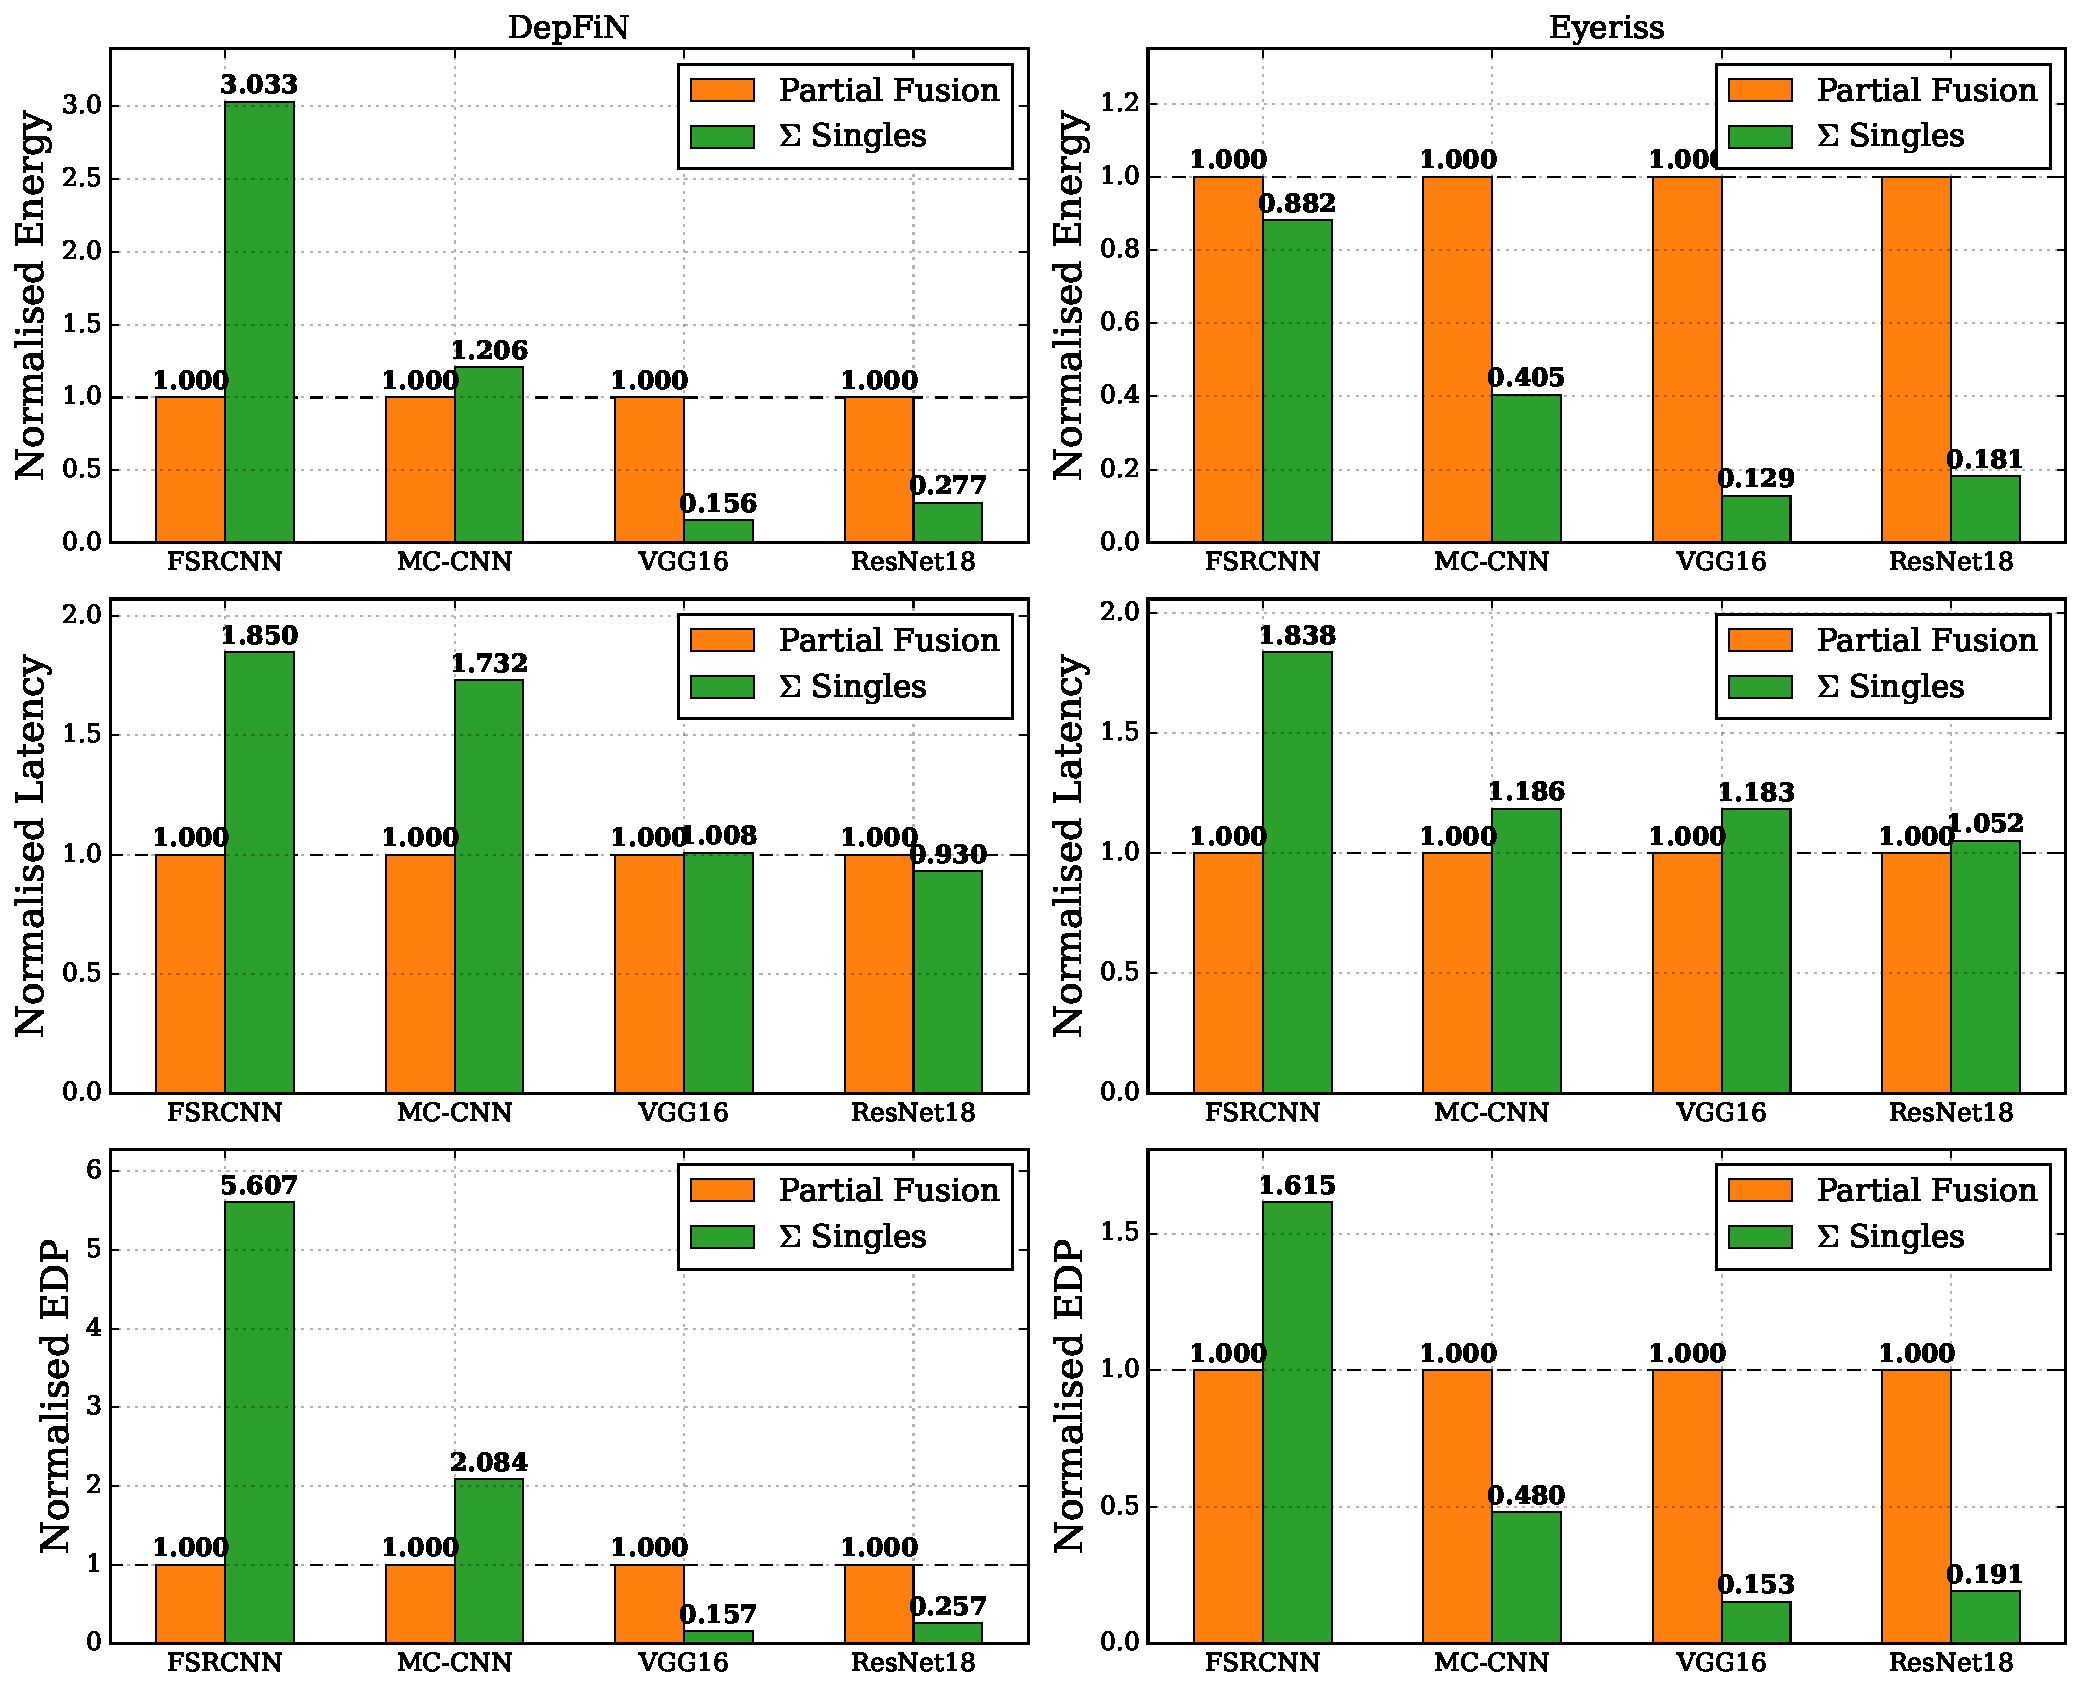
\includegraphics[width=0.95\textwidth]{plots/fusion_partial_sized_norm.pdf}
  \caption{Scenario~B — Normalised energy (top), latency (middle),
    and EDP (bottom), with partial fusion\,=\,1.0.
    Bars below 1.0 indicate the single-layer sum is more efficient.}
  \label{fig:partial-sized-norm}
\end{figure}

\paragraph{Comparison with Scenario~A.}
Scenario~B demonstrates that sizing the architecture for pairwise
fusion rather than full fusion brings two clear advantages.

The first is the substantial memory reduction
(Table~\ref{tab:partial-sized-configs}), which lowers energy cost access for the memories and registers.
The second is that the latency benefit of fusion is almost fully
preserved: partial fusion captures $96$--$100\%$ of the
full-fusion latency saving for the activation-dominant workloads,
and it eliminates or greatly reduces the worst-case latency
penalty that full fusion imposed on DepFiN
($-11.3\%{\to}+0.8\%$ for VGG16; $-30.3\%{\to}-7.5\%$ for
ResNet18).


The EDP verdict is identical in scope: three of eight
architecture--workload combinations favor fusion in both
scenarios (FSRCNN and MC-CNN on DepFiN, FSRCNN on Eyeriss).
The weight-dominant workloads continue to favor single-layer
execution on both architectures, regardless of whether the
design targets full or partial fusion.

\paragraph{Considerations}
A partial-fusion-sized architecture delivers nearly the same
latency and EDP benefit as a full-fusion architecture, at a
fraction of the memory cost.
For activation-dominant workloads on DepFiN, partial fusion
wins on energy, latency, and EDP simultaneously, making it
the strictly dominant strategy.
On Eyeriss, partial fusion wins on EDP only for the most
activation-heavy workload (FSRCNN), because the replicated
register overhead partially offsets the DRAM savings.
For weight-dominant workloads, the on-chip memory overhead of
fusion still outweighs the DRAM savings,
and single-layer execution remains the more efficient choice
on both architectures.
